\chapter{时间复杂度}

\index{时间复杂度}

在竞赛编程中，算法的效率非常重要。
通常，设计一个能够解决问题但速度较慢的算法是容易的，
真正的挑战在于发明一个高效的算法。
如果算法太慢，将只能得到部分分数，甚至完全得不到分数。

算法的\key{时间复杂度}用于估计算法在处理某种输入时所需的时间。
其核心思想是将效率表示为一个函数，该函数的参数是输入的大小。
通过计算时间复杂度，
我们可以在不实现算法的情况下判断它是否足够快。

\section{计算规则}

算法的时间复杂度记为$O(\cdots)$，
其中三个点代表某个函数。
通常，变量$n$表示输入大小。
例如，如果输入是一个数字数组，
$n$就是数组的大小；
如果输入是一个字符串，
$n$就是字符串的长度。

\subsubsection*{循环}

算法慢的一个常见原因是它包含许多遍历输入的循环。
算法中嵌套的循环越多，速度就越慢。
如果有$k$层嵌套循环，
时间复杂度为$O(n^k)$。

例如，以下代码的时间复杂度为$O(n)$：
\begin{lstlisting}
for (int i = 1; i <= n; i++) {
    // 代码
}
\end{lstlisting}

而以下代码的时间复杂度为$O(n^2)$：
\begin{lstlisting}
for (int i = 1; i <= n; i++) {
    for (int j = 1; j <= n; j++) {
        // 代码
    }
}
\end{lstlisting}

\subsubsection*{数量级}

时间复杂度并不能告诉我们循环内部的代码被执行的确切次数，
它只显示了数量级。
在以下示例中，循环内部的代码
分别执行$3n$、$n+5$和$\lceil n/2 \rceil$次，
但每段代码的时间复杂度都是$O(n)$。

\begin{lstlisting}
for (int i = 1; i <= 3*n; i++) {
    // 代码
}
\end{lstlisting}

\begin{lstlisting}
for (int i = 1; i <= n+5; i++) {
    // 代码
}
\end{lstlisting}

\begin{lstlisting}
for (int i = 1; i <= n; i += 2) {
    // 代码
}
\end{lstlisting}

再看另一个例子，
以下代码的时间复杂度为$O(n^2)$：

\begin{lstlisting}
for (int i = 1; i <= n; i++) {
    for (int j = i+1; j <= n; j++) {
        // 代码
    }
}
\end{lstlisting}

\subsubsection*{阶段}

如果算法由连续的阶段组成，
总时间复杂度就是单个阶段中最大的时间复杂度。
原因是最慢的阶段通常是代码的瓶颈。

例如，以下代码由三个阶段组成，
时间复杂度分别为$O(n)$、$O(n^2)$和$O(n)$。
因此，总时间复杂度为$O(n^2)$。

\begin{lstlisting}
for (int i = 1; i <= n; i++) {
    // 代码
}
for (int i = 1; i <= n; i++) {
    for (int j = 1; j <= n; j++) {
        // 代码
    }
}
for (int i = 1; i <= n; i++) {
    // 代码
}
\end{lstlisting}

\subsubsection*{多个变量}

有时时间复杂度取决于多个因素。
在这种情况下，时间复杂度公式中会包含多个变量。

例如，以下代码的时间复杂度为$O(nm)$：

\begin{lstlisting}
for (int i = 1; i <= n; i++) {
    for (int j = 1; j <= m; j++) {
        // 代码
    }
}
\end{lstlisting}

\subsubsection*{递归}

递归函数的时间复杂度取决于函数被调用的次数
以及单次调用的时间复杂度。
总时间复杂度是这两个值的乘积。

例如，考虑以下函数：
\begin{lstlisting}
void f(int n) {
    if (n == 1) return;
    f(n-1);
}
\end{lstlisting}
调用$\texttt{f}(n)$会产生$n$次函数调用，
而每次调用的时间复杂度为$O(1)$。
因此，总时间复杂度为$O(n)$。

再看另一个例子，考虑以下函数：
\begin{lstlisting}
void g(int n) {
    if (n == 1) return;
    g(n-1);
    g(n-1);
}
\end{lstlisting}
在这种情况下，除了$n=1$外，每次函数调用都会生成另外两次调用。
让我们看看当$g$以参数$n$被调用时会发生什么。
下表显示了由这一次调用产生的函数调用：
\begin{center}
\begin{tabular}{rr}
函数调用 & 调用次数 \\
\hline
$g(n)$ & 1 \\
$g(n-1)$ & 2 \\
$g(n-2)$ & 4 \\
$\cdots$ & $\cdots$ \\
$g(1)$ & $2^{n-1}$ \\
\end{tabular}
\end{center}
据此，时间复杂度为
\[1+2+4+\cdots+2^{n-1} = 2^n-1 = O(2^n).\]

\section{复杂度类别}

\index{复杂度类别}

以下列表包含算法常见的各种时间复杂度：

\begin{description}
\item[$O(1)$]
\index{常数时间算法}
\key{常数时间}算法的运行时间不依赖于输入大小。
典型的常数时间算法是一个直接计算答案的公式。

\item[$O(\log n)$]
\index{对数算法}
\key{对数}算法通常在每一步将输入大小减半。
这类算法的运行时间是对数级的，因为
$\log_2 n$等于$n$
需要除以2多少次才能得到1。

\item[$O(\sqrt n)$]
\key{平方根算法}比$O(\log n)$慢，
但比$O(n)$快。
平方根的一个特殊性质是
$\sqrt n = n/\sqrt n$，所以平方根$\sqrt n$在某种意义上
位于输入的中间位置。

\item[$O(n)$]
\index{线性算法}
\key{线性}算法以常数次遍历输入。
这通常是可能达到的最好时间复杂度，
因为在报告答案之前，通常需要至少访问每个输入元素一次。

\item[$O(n \log n)$]
这种时间复杂度通常意味着算法对输入进行了排序，
因为高效排序算法的时间复杂度为$O(n \log n)$。
另一种可能是算法使用了一种数据结构，
其中每个操作需要$O(\log n)$的时间。

\item[$O(n^2)$]
\index{平方算法}
\key{平方}算法通常包含两层嵌套循环。
可以在$O(n^2)$时间内遍历所有输入元素的对。

\item[$O(n^3)$]
\index{立方算法}
\key{立方}算法通常包含三层嵌套循环。
可以在$O(n^3)$时间内遍历所有输入元素的三元组。

\item[$O(2^n)$]
这种时间复杂度通常意味着算法遍历了输入元素的所有子集。
例如，$\{1,2,3\}$的子集有
$\emptyset$、$\{1\}$、$\{2\}$、$\{3\}$、$\{1,2\}$、
$\{1,3\}$、$\{2,3\}$和$\{1,2,3\}$。

\item[$O(n!)$]
这种时间复杂度通常意味着算法遍历了输入元素的所有排列。
例如，$\{1,2,3\}$的排列有
$(1,2,3)$、$(1,3,2)$、$(2,1,3)$、$(2,3,1)$、
$(3,1,2)$和$(3,2,1)$。

\end{description}

\index{多项式算法}
如果一个算法的时间复杂度最多为$O(n^k)$，
其中$k$是一个常数，则该算法是\key{多项式}的。
除$O(2^n)$和$O(n!)$外，
上述所有时间复杂度都是多项式的。
在实际应用中，常数$k$通常很小，
因此多项式时间复杂度大致意味着算法是\emph{高效的}。

\index{NP-hard问题}

本书中大多数算法都是多项式的。
尽管如此，仍有许多重要问题没有已知的多项式算法，
也就是说，没有人知道如何高效地解决它们。
\key{NP-hard}问题是一类重要的问题集，
对于这些问题目前还没有已知的多项式算法\footnote{关于这一主题的经典著作是
M. R. Garey和D. S. Johnson的
\emph{Computers and Intractability: A Guide to the Theory
of NP-Completeness} \cite{gar79}。}。

\section{估算效率}

通过计算算法的时间复杂度，
可以在实现算法之前检查它是否足够高效地解决问题。
估算的出发点是一个事实：
现代计算机可以在一秒钟内执行数亿次操作。

例如，假设某个问题的时间限制是一秒，输入大小为$n=10^5$。
如果时间复杂度是$O(n^2)$，
算法将执行约$(10^5)^2=10^{10}$次操作。
这至少需要数十秒的时间，
因此该算法似乎太慢了，无法解决该问题。

另一方面，给定输入大小，
我们可以尝试\emph{猜测}
解决该问题的算法所需的时间复杂度。
下表包含一些有用的估算，
假设时间限制为一秒。

\begin{center}
\begin{tabular}{ll}
输入大小 & 所需时间复杂度 \\
\hline
$n \le 10$ & $O(n!)$ \\
$n \le 20$ & $O(2^n)$ \\
$n \le 500$ & $O(n^3)$ \\
$n \le 5000$ & $O(n^2)$ \\
$n \le 10^6$ & $O(n \log n)$或$O(n)$ \\
$n$很大 & $O(1)$或$O(\log n)$ \\
\end{tabular}
\end{center}

例如，如果输入大小为$n=10^5$，
可能期望算法的时间复杂度为$O(n)$或$O(n \log n)$。
这个信息使得设计算法更容易，
因为它排除了那些会产生更差时间复杂度的方法。

\index{常数因子}

不过，重要的是要记住，
时间复杂度只是对效率的估算，
因为它隐藏了\emph{常数因子}。
例如，运行时间为$O(n)$的算法
可能执行$n/2$或$5n$次操作。
这对算法的实际运行时间有重要影响。

\section{最大子数组和}

\index{最大子数组和}

通常有几种不同的算法可以解决同一个问题，
它们的时间复杂度各不相同。
本节讨论一个经典问题，
它有一个直观的$O(n^3)$解法。
然而，通过设计更好的算法，
可以在$O(n^2)$时间内解决该问题，
甚至在$O(n)$时间内解决。

给定一个包含$n$个数的数组，
我们的任务是计算\key{最大子数组和}，即
数组中连续值序列的最大可能和\footnote{J. Bentley的
著作\emph{Programming Pearls} \cite{ben86}使这个问题广为人知。}。
当数组中可能存在负数时，这个问题才有趣。
例如，在数组
\begin{center}
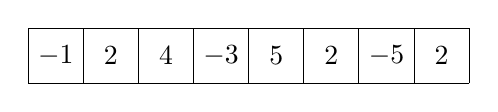
\begin{tikzpicture}[scale=0.7]
\draw (0,0) grid (8,1);

\node at (0.5,0.5) {$-1$};
\node at (1.5,0.5) {$2$};
\node at (2.5,0.5) {$4$};
\node at (3.5,0.5) {$-3$};
\node at (4.5,0.5) {$5$};
\node at (5.5,0.5) {$2$};
\node at (6.5,0.5) {$-5$};
\node at (7.5,0.5) {$2$};
\end{tikzpicture}
\end{center}
\begin{samepage}
以下子数组产生了最大和$10$：
\begin{center}
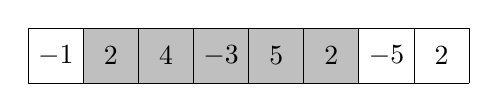
\begin{tikzpicture}[scale=0.7]
\fill[color=lightgray] (1,0) rectangle (6,1);
\draw (0,0) grid (8,1);

\node at (0.5,0.5) {$-1$};
\node at (1.5,0.5) {$2$};
\node at (2.5,0.5) {$4$};
\node at (3.5,0.5) {$-3$};
\node at (4.5,0.5) {$5$};
\node at (5.5,0.5) {$2$};
\node at (6.5,0.5) {$-5$};
\node at (7.5,0.5) {$2$};
\end{tikzpicture}
\end{center}
\end{samepage}

我们假设允许空子数组，
因此最大子数组和总是至少为$0$。

\subsubsection{算法1}

解决问题的一种直观方法是遍历所有可能的子数组，
计算每个子数组的值之和，并维护最大和。
以下代码实现了这个算法：

\begin{lstlisting}
int best = 0;
for (int a = 0; a < n; a++) {
    for (int b = a; b < n; b++) {
        int sum = 0;
        for (int k = a; k <= b; k++) {
            sum += array[k];
        }
        best = max(best,sum);
    }
}
cout << best << "\n";
\end{lstlisting}

变量\texttt{a}和\texttt{b}固定了子数组的
第一个和最后一个索引，
值之和计算到变量\texttt{sum}中。
变量\texttt{best}包含搜索过程中找到的最大和。

该算法的时间复杂度为$O(n^3)$，
因为它由三个遍历输入的嵌套循环组成。

\subsubsection{算法2}

通过去掉一个循环，很容易让算法1变得更高效。
这可以通过在子数组右端移动的同时计算和来实现。
结果如下代码：

\begin{lstlisting}
int best = 0;
for (int a = 0; a < n; a++) {
    int sum = 0;
    for (int b = a; b < n; b++) {
        sum += array[b];
        best = max(best,sum);
    }
}
cout << best << "\n";
\end{lstlisting}
这一改变后，时间复杂度为$O(n^2)$。

\subsubsection{算法3}

令人惊讶的是，可以在$O(n)$时间内解决该问题\footnote{在\cite{ben86}中，这个线性时间算法被归功于J. B. Kadane，
因此该算法有时被称为\index{Kadane算法} \key{Kadane算法}。}，这意味着只需一个循环即可。
其思想是，对于每个数组位置，
计算以该位置结尾的子数组的最大和。
之后，问题的答案就是这些和中的最大值。

考虑寻找以位置$k$结尾的最大和子数组的子问题。
有两种可能：
\begin{enumerate}
\item 子数组只包含位置$k$处的元素。
\item 子数组由一个以位置$k-1$结尾的子数组
加上位置$k$处的元素组成。
\end{enumerate}

在后者的情况下，由于我们要找到
和最大的子数组，
以位置$k-1$结尾的子数组也应该是和最大的。
因此，我们可以通过从左到右计算每个结束位置的最大子数组和，
来高效地解决问题。

以下代码实现了该算法：
\begin{lstlisting}
int best = 0, sum = 0;
for (int k = 0; k < n; k++) {
    sum = max(array[k],sum+array[k]);
    best = max(best,sum);
}
cout << best << "\n";
\end{lstlisting}

该算法只包含一个遍历输入的循环，
因此时间复杂度为$O(n)$。
这也是可能达到的最好时间复杂度，
因为解决该问题的任何算法
都必须至少检查所有数组元素一次。

\subsubsection{效率比较}

研究算法在实践中有多高效是很有趣的。
下表展示了上述算法在现代计算机上
对于不同$n$值的运行时间。

在每次测试中，输入是随机生成的。
读取输入所需的时间未被测量。

\begin{center}
\begin{tabular}{rrrr}
数组大小$n$ & 算法1 & 算法2 & 算法3 \\
\hline
$10^2$ & $0.0$秒 & $0.0$秒 & $0.0$秒 \\
$10^3$ & $0.1$秒 & $0.0$秒 & $0.0$秒 \\
$10^4$ & > $10.0$秒 & $0.1$秒 & $0.0$秒 \\
$10^5$ & > $10.0$秒 & $5.3$秒 & $0.0$秒 \\
$10^6$ & > $10.0$秒 & > $10.0$秒 & $0.0$秒 \\
$10^7$ & > $10.0$秒 & > $10.0$秒 & $0.0$秒 \\
\end{tabular}
\end{center}

比较结果显示，当输入大小较小时，
所有算法都是高效的，
但随着输入增大，算法之间的运行时间
会出现显著差异。
当$n=10^4$时，算法1变慢；
当$n=10^5$时，算法2变慢。
只有算法3能够瞬间处理
即使是最大的输入。
